\documentclass[border=10pt]{standalone}
\usepackage[svgnames]{xcolor}
\usepackage{amsmath}
\usepackage{pgfplots}
\pgfplotsset{compat=newest}
\usepackage[sfdefault]{FiraSans}
\usepackage{FiraMono}
\renewcommand*\familydefault{\sfdefault}
\begin{document}
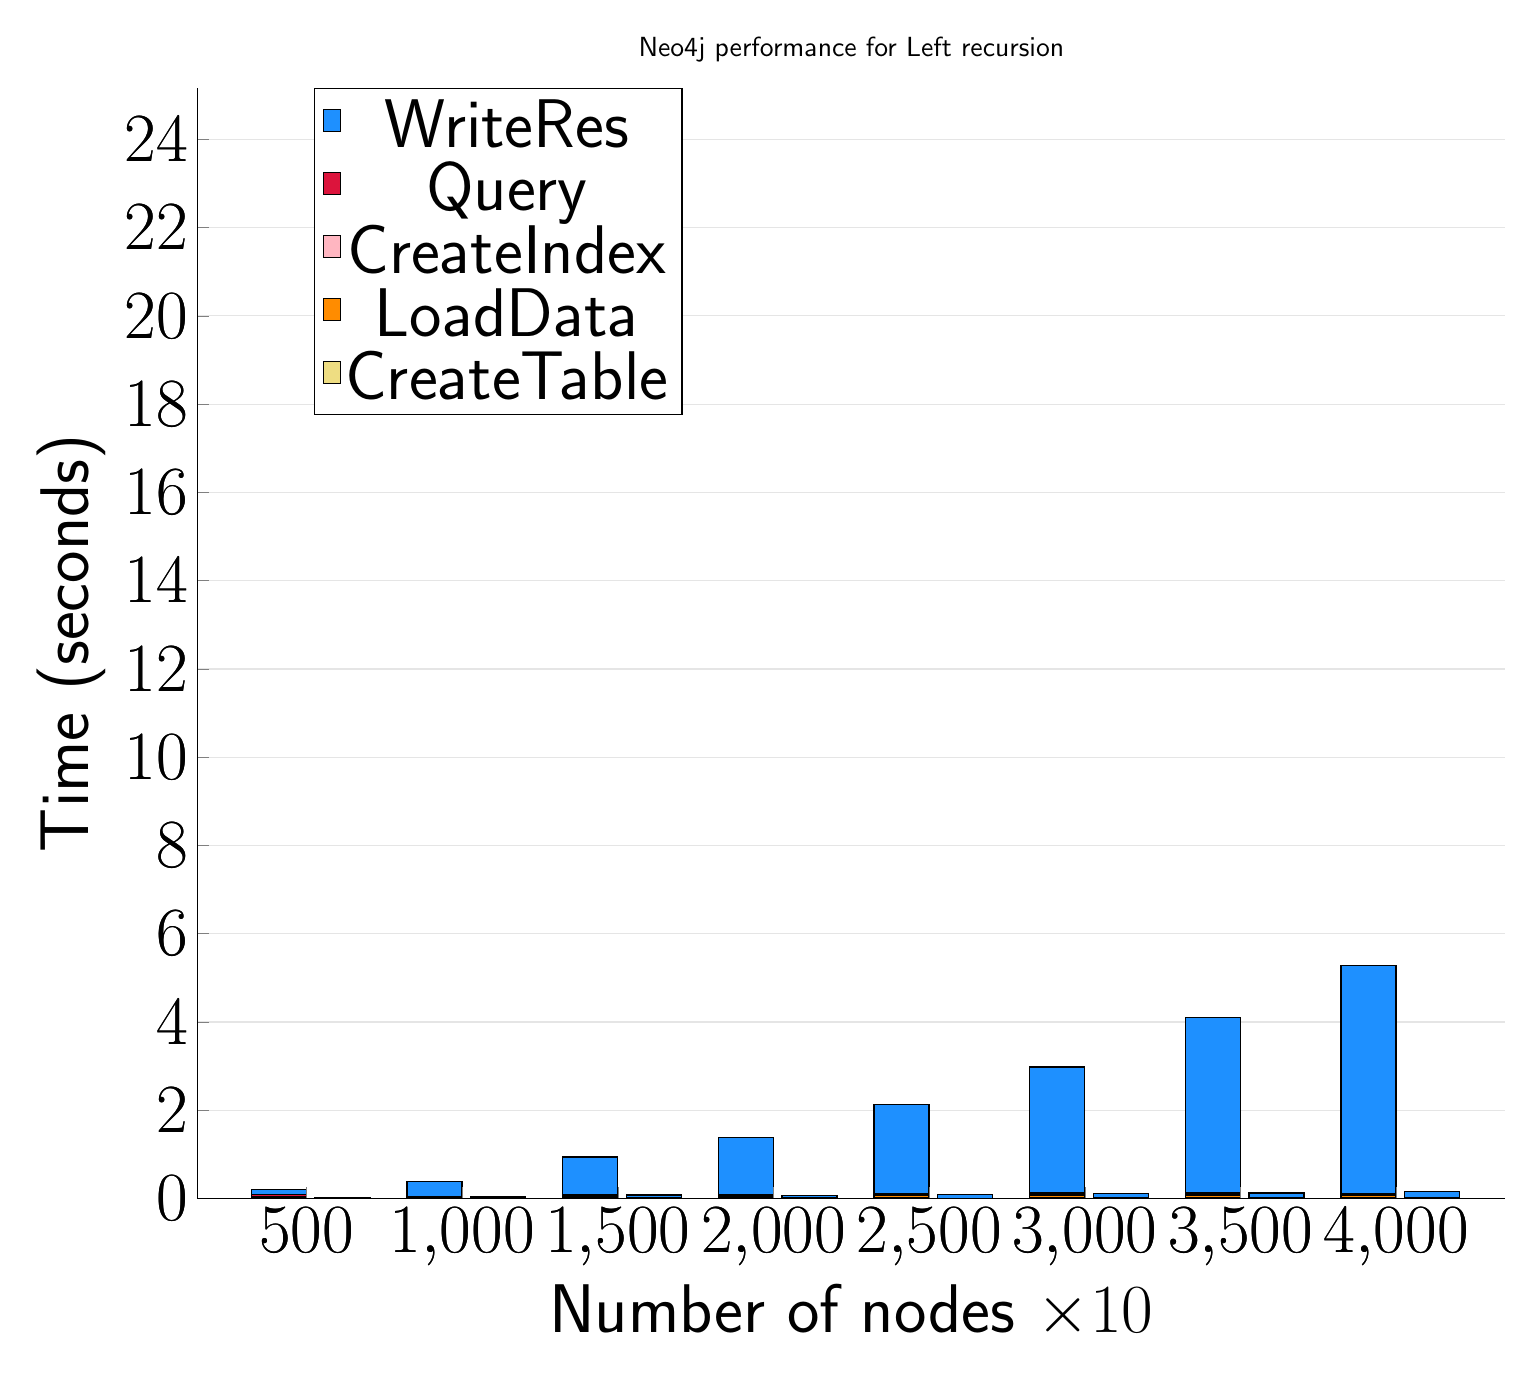
\begin{tikzpicture}
\begin{axis}[
   ybar stacked,
   title={Neo4j performance for Left recursion},
   bar shift=-10pt,
   width=1.5\textwidth,
   bar width=0.7cm,
   ymajorgrids, tick align=inside,
   major grid style={draw=gray!20},
   xtick=data,
   ymin=0, ymax=25.16666666418314,
   axis x line*=bottom,
   axis y line*=left,
   enlarge x limits=0.1,
   legend style={
       at={(0.23, 1)},
       anchor=north,
       legend columns=1,
       font=\Huge,
   },
   ylabel={Time (seconds)},
   xlabel={Number of nodes $\times 10$},
   label style={font=\Huge},
   tick label style={font=\Huge},
]
\addlegendimage{fill=DodgerBlue, draw=black, line width=0.2pt}
\addlegendentry{WriteRes}
\addlegendimage{fill=Crimson, draw=black, line width=0.2pt}
\addlegendentry{Query}
\addlegendimage{fill=LightPink, draw=black, line width=0.2pt}
\addlegendentry{CreateIndex}
\addlegendimage{fill=DarkOrange, draw=black, line width=0.2pt}
\addlegendentry{LoadData}
\addlegendimage{fill=LightGoldenrod, draw=black, line width=0.2pt}
\addlegendentry{CreateTable}
\addplot +[fill=LightGoldenrod, draw=black, line width=0.5pt] coordinates {
    (500, 0.01333333303531011)
    (1000, 0.010000000397364298)
    (1500, 0.016666668156782787)
    (2000, 0.01666666567325592)
    (2500, 0.013333330551783243)
    (3000, 0.020000003278255463)
    (3500, 0.013333330551783243)
    (4000, 0.019999995827674866)
};
\addplot +[fill=DarkOrange, draw=black, line width=0.5pt] coordinates {
    (500, 0.023333335916201275)
    (1000, 0.02666666607062022)
    (1500, 0.04000000158945719)
    (2000, 0.033333333830038704)
    (2500, 0.07000000029802322)
    (3000, 0.06333333253860474)
    (3500, 0.0633333350221316)
    (4000, 0.0633333350221316)
};
\addplot +[fill=LightPink, draw=black, line width=0.5pt] coordinates {
    (500, 0.013333330551783243)
    (1000, 0.01666667064030965)
    (1500, 0.02333333094914754)
    (2000, 0.020000000794728596)
    (2500, 0.030000001192092896)
    (3000, 0.033333333830038704)
    (3500, 0.03999999910593033)
    (4000, 0.03666666646798452)
};
\addplot +[fill=Crimson, draw=black, line width=0.5pt] coordinates {
    (500, 0.03666666646798452)
    (1000, 0.0)
    (1500, 0.0066666677594184875)
    (2000, 0.023333333432674408)
    (2500, 0.006666665275891622)
    (3000, 0.006666665275891622)
    (3500, 0.0066666677594184875)
    (4000, 0.0)
};
\addplot +[fill=DodgerBlue, draw=black, line width=0.5pt] coordinates {
    (500, 0.11333333452542622)
    (1000, 0.339999998609225)
    (1500, 0.8566666692495346)
    (2000, 1.2899999991059303)
    (2500, 2.0066666652758918)
    (3000, 2.8599999994039536)
    (3500, 3.983333334326744)
    (4000, 5.16666666418314)
};
\end{axis}
\begin{axis}[
   ybar stacked,
   bar shift=13pt,
   width=1.5\textwidth,
   bar width=0.7cm,
   ymajorgrids, tick align=inside,
   major grid style={draw=none},
   xtick=data,
   ymin=0, ymax=25.16666666418314,
   axis x line*=none,
   axis y line*=none,
   enlarge x limits=0.1,
   label style={font=\Huge},
   tick label style={font=\Huge},
]
\addplot +[fill=LightGoldenrod, draw=black, line width=0.5pt] coordinates {
    (500, 0.013333333333333324)
    (1000, 0.003333333333333337)
    (1500, 0.013333333333333341)
    (2000, 0.006666666666666637)
    (2500, 0.006666666666666672)
    (3000, 0.006666666666666636)
    (3500, 0.00999999999999999)
    (4000, 0.0033333333333333184)
};
\addplot +[fill=DarkOrange, draw=black, line width=0.5pt] coordinates {
    (500, 0.0)
    (1000, 0.0)
    (1500, 0.0)
    (2000, 0.0)
    (2500, 0.0)
    (3000, 0.0)
    (3500, 0.0)
    (4000, 0.003333333333333318)
};
\addplot +[fill=LightPink, draw=black, line width=0.5pt] coordinates {
    (500, 0.0)
    (1000, 0.006666666666666674)
    (1500, 0.0)
    (2000, 0.0)
    (2500, 0.0)
    (3000, 0.0)
    (3500, 0.0)
    (4000, 0.003333333333333336)
};
\addplot +[fill=Crimson, draw=black, line width=0.5pt] coordinates {
    (500, 0.0)
    (1000, 0.0)
    (1500, 0.006666666666666668)
    (2000, 0.0033333333333333344)
    (2500, 0.0)
    (3000, 0.006666666666666669)
    (3500, 0.003333333333333336)
    (4000, 0.0)
};
\addplot +[fill=DodgerBlue, draw=black, line width=0.5pt] coordinates {
    (500, 0.01666666666666666)
    (1000, 0.033333333333333354)
    (1500, 0.056666666666666664)
    (2000, 0.06)
    (2500, 0.07999999999999999)
    (3000, 0.10333333333333335)
    (3500, 0.11333333333333336)
    (4000, 0.1466666666666667)
};
\end{axis}
\end{tikzpicture}

\end{document}
